\documentclass[tikz,border=2pt]{standalone}
\usepackage{amsmath}
\usetikzlibrary{arrows.meta,decorations.pathreplacing}
\begin{document}
% cond = (1:5 > 2) & (1:5 < 5) = F F T T F, read as 0 0 1 1 0:
% sum = 2, mean = 0.4, any = TRUE, all = FALSE.
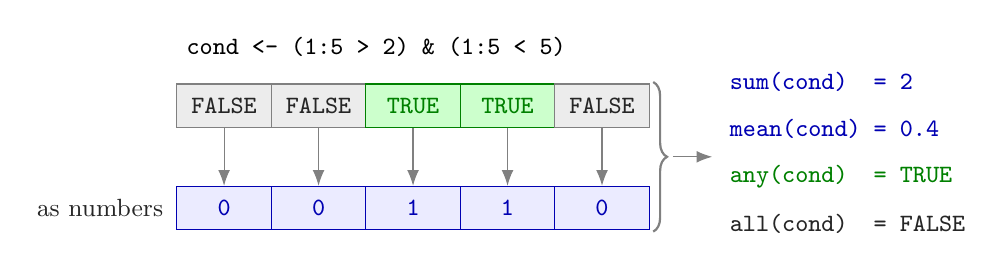
\begin{tikzpicture}[font=\small, >={Latex[length=2mm]},
  cell/.style={draw, minimum width=1.2cm, minimum height=0.55cm, inner sep=1pt, font=\small\ttfamily},
  yes/.style={cell, draw=green!50!black, fill=green!20, text=green!50!black},
  no/.style={cell, draw=gray, fill=gray!15, text=gray!30!black},
  num/.style={cell, draw=blue!70!black, fill=blue!8, text=blue!70!black},
  res/.style={anchor=west, font=\small\ttfamily}]
  \node[anchor=west, font=\small\ttfamily] at (0.6,0.75) {cond <- (1:5 > 2) \& (1:5 < 5)};
  \foreach \s/\t [count=\i] in {no/FALSE,no/FALSE,yes/TRUE,yes/TRUE,no/FALSE} {
    \node[\s] (a\i) at (1.2*\i,0) {\t};
  }
  \foreach \v [count=\i] in {0,0,1,1,0} {
    \node[num] (b\i) at (1.2*\i,-1.3) {\v};
    \draw[->, gray] (a\i.south) -- (b\i.north);
  }
  \node[anchor=east, gray!30!black] at (0.55,-1.3) {as numbers};
  \draw[decorate, decoration={brace, amplitude=5pt}, thick, gray] (6.65,0.3) -- (6.65,-1.6);
  \draw[->, gray] (6.9,-0.65) -- (7.4,-0.65);
  \node[res, blue!70!black]  at (7.5,0.3)  {sum(cond)\ \ = 2};
  \node[res, blue!70!black]  at (7.5,-0.3) {mean(cond) = 0.4};
  \node[res, green!50!black] at (7.5,-0.9) {any(cond)\ \ = TRUE};
  \node[res, gray!30!black]  at (7.5,-1.5) {all(cond)\ \ = FALSE};
\end{tikzpicture}
\end{document}
